%Beschreibung der Implementierung der Kommunikation mit & Auswertung der Werte von dem Gyro

\subsection{Hardware}
Für die Ermittlung der Ausrichtung des Würfels wurde ein digitaler Beschleunigungsmesser verwendet. Für das Projekt standen anfangs zwei Geräte zur Verfügung: BNO055 von Adafruit und ADXL345 von Analog Devices. Zwar ist der Beschleunigungsmesser von Adafruit mächtiger, da dieser mehr Messungen vornimmt und eine größere Genauigkeit ermöglicht, dennoch wurde das Projekt am Ende unter der Verwendung des Beschleunigungsmessers ADXL345 umgesetzt. Grund dafür war, dass nach mehreren Versuchen mit dem Gerät von Adafruit zu kommunizieren festgestellt wurde, dass der Beschleunigungsmesser nicht defekt war. In alle Registern des Bausteins anstatt der vorprogrammierte Daten liegt nur die Zahl \texttt{0xE5}, was laut dem Hersteller zeigt, dass die Registern beim Startup nicht geleert werden.

Für die Verwendung des ADXL345 sollte man in Programm nur die Adressen ändern und richtig alle Pins belegen. Die ALT ADDRESS wurde auf 1 gesetzt und die 7-Bit-I2C-Adresse für das Gerät wurde somit als \texttt{0x1D} festgelegt. In Programm wurde direkt die entsprechende 8-Bit-I2C-Adresse \texttt{0x3A} verwendet und die notwendige Änderung der Adresse in \texttt{0x3B} aus \texttt{0x3A} wurde gerade in I2C Routine erledigt. So kann man unterscheiden, ob es Lesen oder Schreiben Operation durchführen sollen werden. 

Es gibt keine internen Pull-Up- oder Pull-Down-Widerstände für nicht verwendete Pins. Daher gibt es keinen bekannten Status oder Standardstatus für den CS- oder ALT ADDRESS-Pin, wenn er potentialfrei bleibt oder nicht verbunden ist. Es ist erforderlich, dass der CS-Pin an VDD  angeschlossen ist und dass der ALT ADDRESS-Pin bei Verwendung von I2C entweder an VDD oder GND angeschlossen ist (wir haben an VDD angeschlossen).

\begin{figure}[!h]
	\centering
	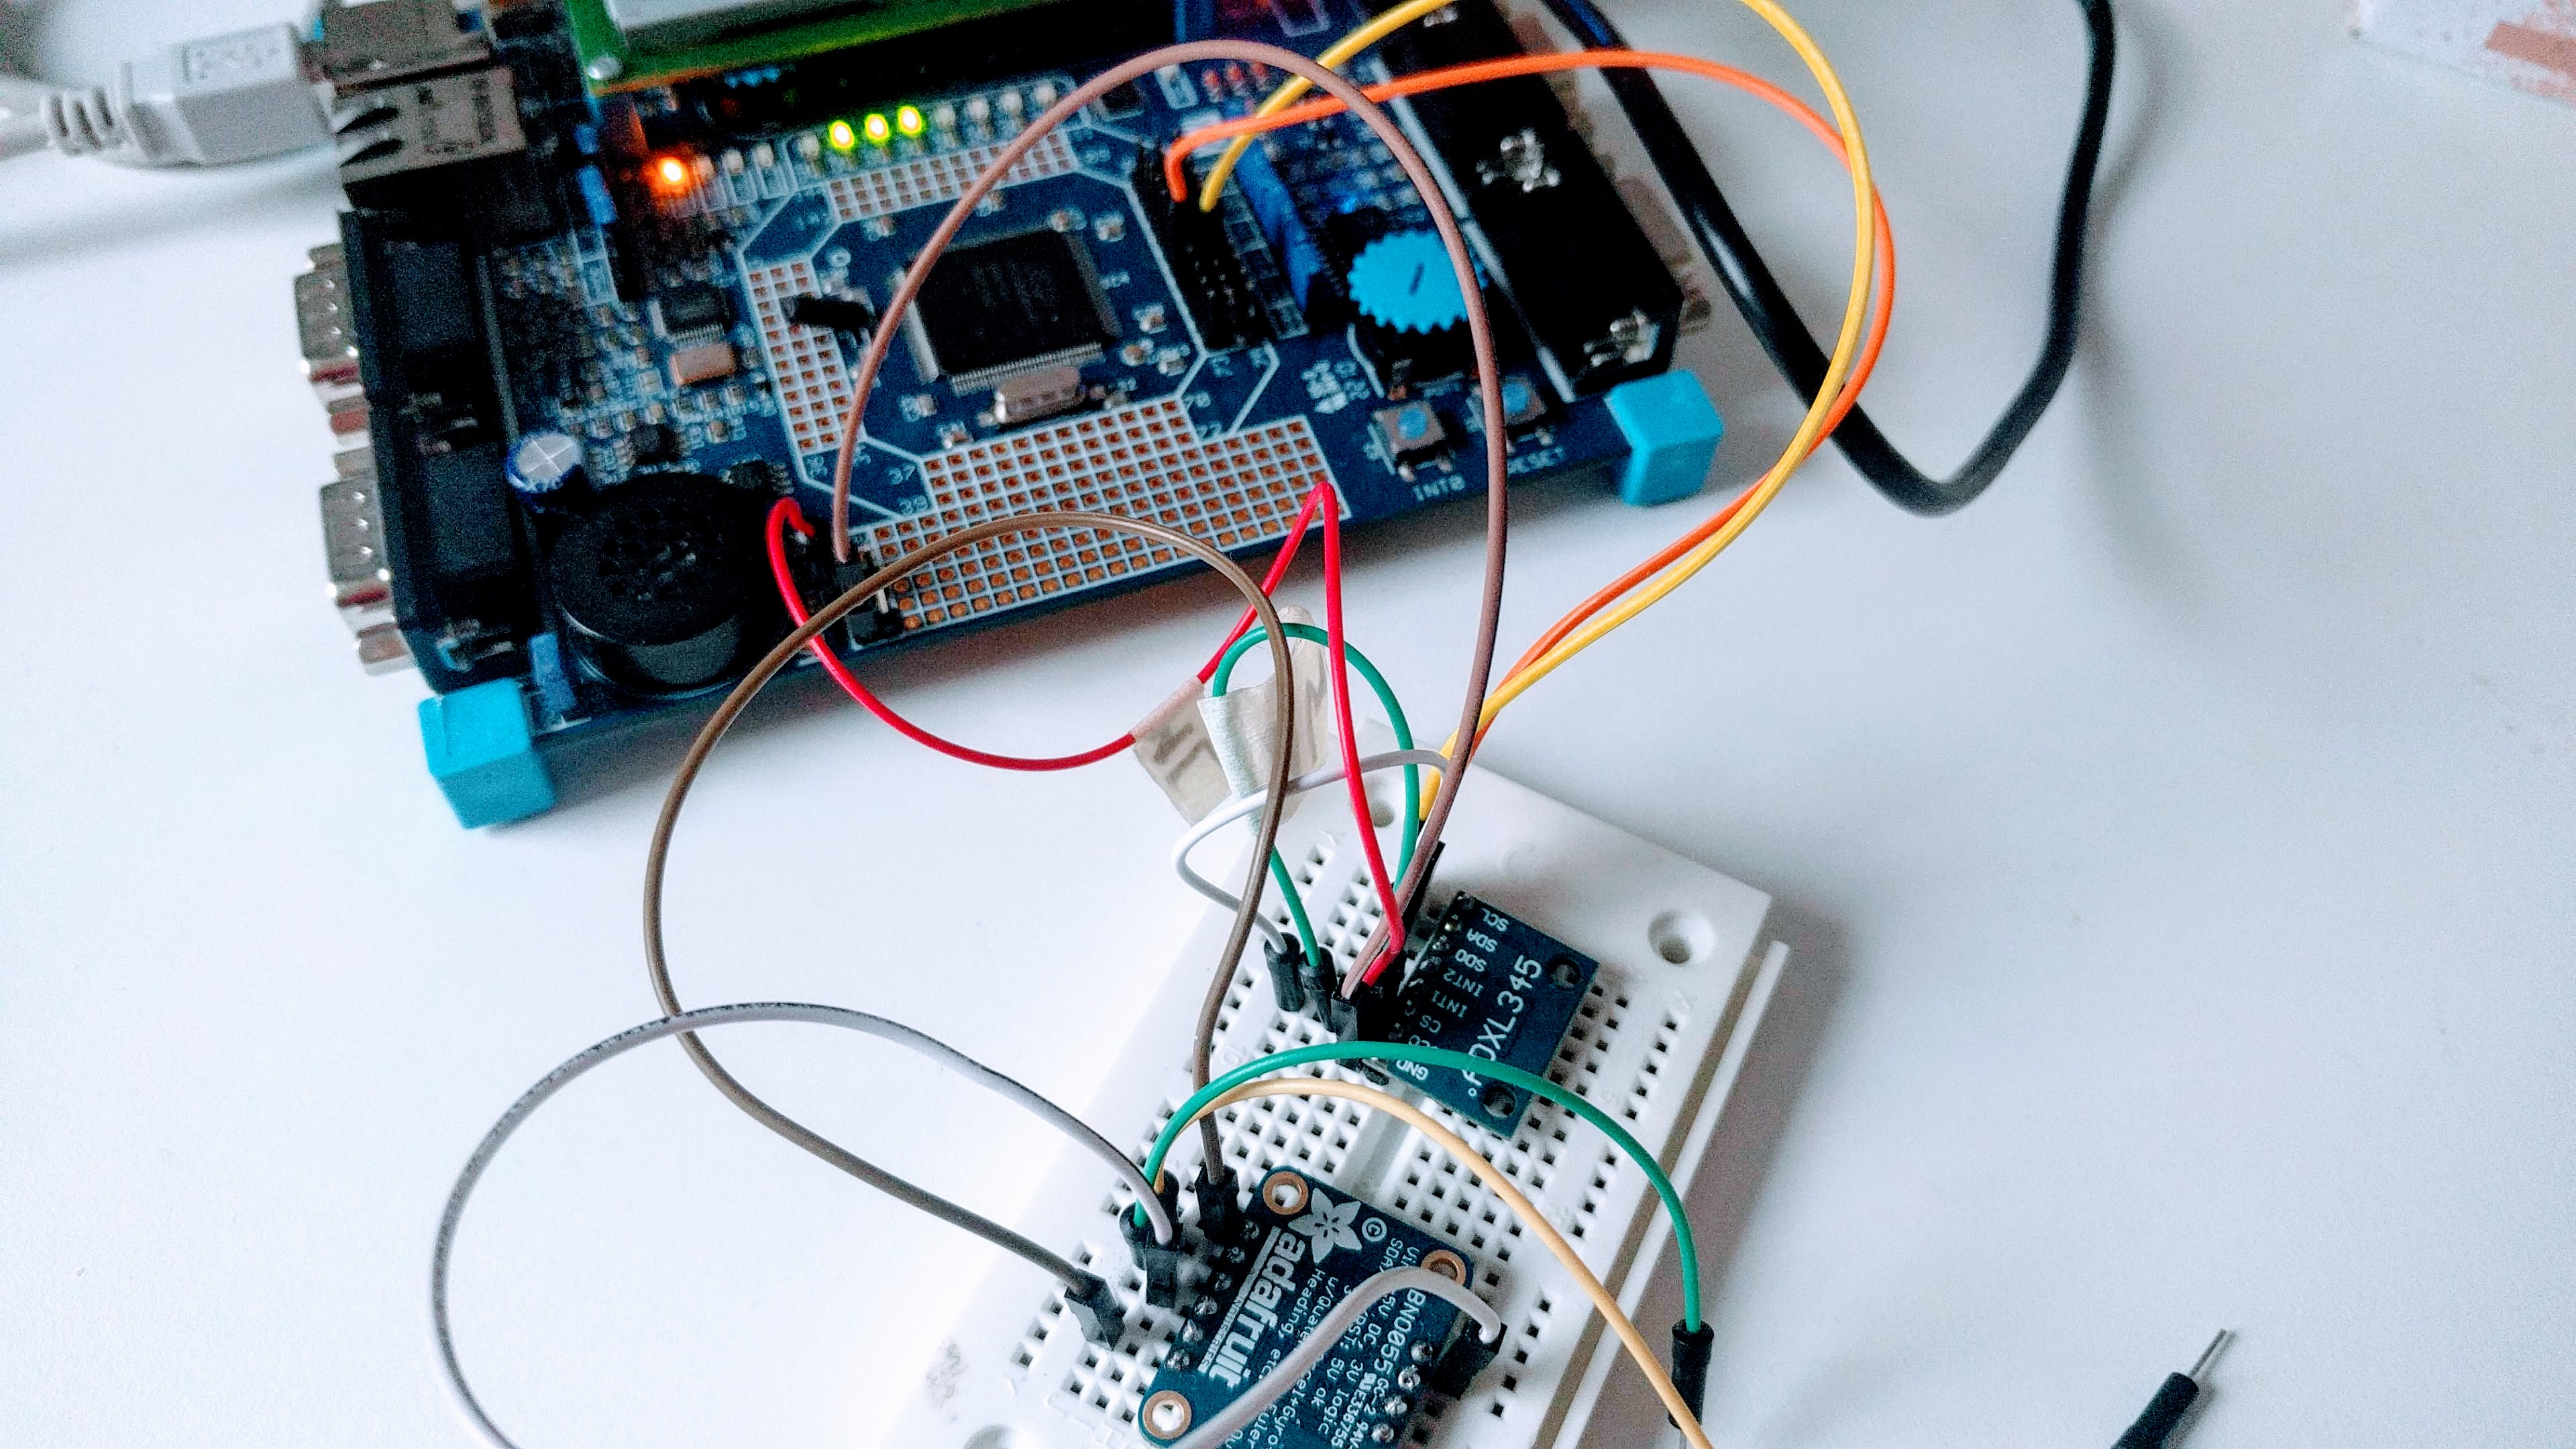
\includegraphics[width=1\linewidth]{adx_wires.jpg}
	\caption[AXL345 Pin Belegung]{ADXL345 Pin Belegung}
	\label{fig:i2cwires}
\end{figure}

Die gemessene Daten werden aus die Register \texttt{0x32} bis Register \texttt{0x37} gelesen. Diese sechs Bytes (Register 0x32 bis Register 0x37) sind jeweils acht Bits und enthalten die Ausgangsdaten für jede Achse. Register \texttt{0x32} und Register \texttt{0x33} enthalten die Ausgangsdaten für die X-Achse, Register \texttt{0x34} und Register \texttt{0x35} die Ausgangsdaten für die Y-Achse und Register 0x36 und Register \texttt{0x37} die Ausgangsdaten für die Z-Achse. 

Die Ausgangsdaten sind zwei Komplemente, mit \texttt{DATAx0} als niedrigstwertigem Byte und DATAx1 als höchstwertigem Byte, wobei X, Y oder Z darstellt. Um die Daten richtig zu lesen, wurde es ein Mehrbyte-Lesen von 2 Register durchgeführt und die Daten aus zwei Lesevorgängen nach dem Lesen als 16-Bit Ausgangsdaten dargestellt. 

\begin{lstlisting}
uint16_t i2c16bit = 0x00;
ReadLenght = 2;
GlobalI2CAddr = addr;
I2CMasterBuffer[0] = regs[0];
I2CMasterBuffer[1] = regs[1];
...
// merge the data from two registers
i2c16bit = i2c16bit | I2CReadBuffer[1]; // [REG0, REG1]: REG1 as MSB
i2c16bit = i2c16bit << 8;

i2c16bit = i2c16bit | I2CReadBuffer[0]; // [REG0, REG1]: REG0 as LSB

\end{lstlisting}

\subsection{I2C: Grundlagen und Realisierung auf dem Keil Board}
Für unseres Projekt haben wir I2C Block auf dem Keil Board in Master-Modus programmiert. Mit Master-Sendermodus werden Daten vom Master (Keil Board) zum Slave (Beschleunigungsmesser) übertragen. So erlaubt uns den Beschleunigungsmesser zu initialisieren. 

Im Master-Empfängermodus werden Daten von einem Slave-Sender empfangen. Nach der Initialisierung des Beschleunigungsmessers wird es immer weiter in diesem Modus gearbeitet, da wir nur ständig die ermittelte Position ablesen wollen. 

Für unseres Projekt haben wir I2C1 Block gewählt. Mithilfe von Schaltbild haben wir festgestellt, welche Pins stehen uns zu Verfügung und sind mit anderen Peripheriefunktionen, die während unseres Projekt notwendig sein könnten, nicht belegt. 

\begin{figure}[!hb]
	\centering
	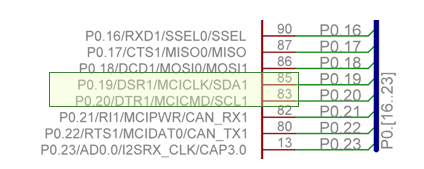
\includegraphics[width=0.6\linewidth]{pins_gyro.jpg}
	\caption[I2C1 Pin Belegung]{2C1 Pin Belegung}
	\label{fig:i2cpins}
	\source{Quelle: \cite{keil.mcb2300}(S. 1)}
\end{figure}

\textbf{START- und STOPP-Bedingungen}. Die I2C-Kommunikation mit diesem Gerät wird initiiert, indem der Master eine START-Bedingung sendet und beendet, indem der Master eine STOP-Bedingung sendet. Ein High-to-Low-Übergang auf der SDA-Leitung, während der SCL-Pegel hoch ist, definiert eine START-Bedingung. Ein Low-to-High-Übergang Die SDA-Leitung definiert die STOP-Bedingung, während der SCL hoch ist. Dies ist mit der folgenden Abbildung\ref{fig:startstop} gezeigt. 

\begin{figure}[!hb]
	\centering
	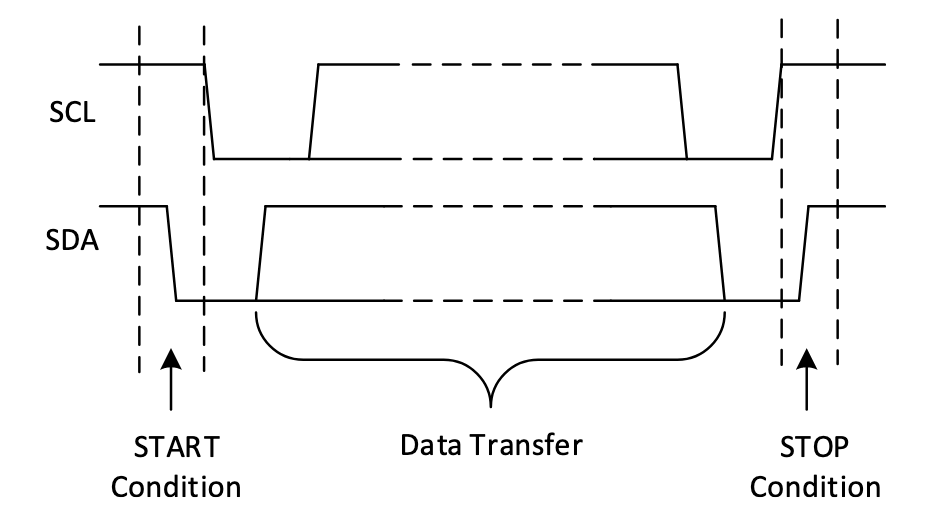
\includegraphics[width=0.6\linewidth]{start_stop.png}
	\caption[I2C Beispiel von START und STOP Bedingungen]{I2C1 Beispiel von START und STOP Bedingungen}
	\label{fig:startstop}
	\source{Quelle: \cite{ti.i2c_bus}(S. 4)}
\end{figure}

Eine \textbf{wiederholte START-Bedingung} sieht ähnlich einer START-Bedingung aus, unterscheidet sich jedoch von einer START-Bedingung, da sie vor einer STOP-Bedingung auftritt (wenn der Bus nicht im Leer ist).

Das \textbf{PCONP}-Register ermöglicht das Deaktivieren ausgewählter Peripheriefunktionen, um Energie zu sparen. Wenn ein Peripheriesteuerbit 1 ist, ist dieses Peripheriegerät aktiviert. Wenn ein Peripherie-Bit 0 ist, wird die Uhr des Peripheriegeräts deaktiviert, um Energie zu sparen. Dem I2C1 entspricht das Bit 19 in PCONP-Register. Um I2C1 zu aktivieren, muss man den Wert $2^{19}$ ins Register schreiben, was in Hexadezimal Format $0x00080000$ entspricht. Mit der Verwendung von logischen Operator $OR$ wird die I2C1 aktiviert und die andere Peripheriefunktionen unverändert geblieben.
\begin{lstlisting}
PCONP |= 0x00080000;
\end{lstlisting}
Die nächste Schritte erlauben es, die Interrupt zu aktivieren. Da dem I2C1 das Bit 19 entspricht, wird es immer mit 19 Bit in jedem Register gearbeitet. \textbf{Vector Address Registers 0-31} (VICVectAddr0-31 sind schreibgeschützte Register. Diese Register enthalten die Adressen der Interrupt-Service-Routinen (ISRs) für die 32 vektorisierten IRQ-Slots.
\begin{lstlisting}
VICVectCntl19 = 0x0000001;   // select a priority slot for interrupt
VICVectAddr19 = (unsigned)i2c_irq; //pass the address of the IRQ
VICIntEnable |= 0x00080000; // enable interrupt
PINSEL1 |= 0x000003C0; //Switch GPIO to I2C pins
\end{lstlisting}

Als nächstes wird ein Auswahl der geeigneten I2C-Datenrate und des Arbeitszyklus durchgeführt. Man muss Werte für die Register \textbf{I2SCLH} und \textbf{I2SCLL} einstellen, um die entsprechende Datenrate und den entsprechenden Arbeitszyklus auszuwählen. I2SCLH definiert die Anzahl der PCLK-Zyklen für die SCL-Hochzeit, I2SCLL definiert die Anzahl der PCLK-Zyklen für die SCL-Niedrigzeit. Dafür wird die folgende Formel benutzt:

\begin{equation}
I^2C_{bitfrequency} =  \frac{F_{PCLK}}{I2SCLH + I2SCLL }
\end{equation}\\

Da es mit der Frequenz von 400KHz gearbeitet wird, wird ins PCONP-Register die entsprechenden Werte geschrieben:
\begin{lstlisting}
I21SCLH = 0xF;
I21SCLL  = 0xF;
\end{lstlisting}

Steuerregister \textbf{I2CONSET} und \textbf{I2CONCLR} enthalten Bits, die zur Steuerung der folgenden I2C-Blockfunktionen verwendet werden: Start und Neustart einer seriellen Übertragung, Beenden einer seriellen Übertragung, Bitrate, Adresserkennung und Bestätigung. Der Inhalt des I2C-Steuerregisters kann als I2CONSET gelesen werden. Beim Schreiben auf I2CONSET werden Bits im I2C-Steuerregister gesetzt, die denen im geschriebenen Wert entsprechen. Umgekehrt löscht das Schreiben in I2CONCLR Bits im I2C-Steuerregister, die denen im geschriebenen Wert entsprechen. Während die Initialisierung wird folgendes in die I2CONSET und I2CONCLR geschrieben: 

\begin{lstlisting}
I21CONCLR = 0x000000FF; // Clear all I2C settings
I21CONSET = 0x00000040; // Enable the I2C interface
\end{lstlisting}

Schieberegister \textbf{I2DAT} enthält ein Byte der zu übertragenden seriellen Daten oder ein gerade empfangenes Byte. Daten in I2DAT werden immer von rechts nach links verschoben. Das erste zu sendende Bit ist das MSB (Bit 7), und nachdem ein Byte empfangen wurde, befindet sich das erste Bit der empfangenen Daten im MSB von I2DAT. 

Der \textbf{Master-Sendermodus} kann jetzt durch Setzen des STA-Bits aufgerufen werden. Die I2C-Logik testet nun den I2C-Bus und generiert eine Startbedingung, sobald der Bus frei wird. Wenn eine START-Bedingung übertragen wird, wird das serielle Interrupt-Flag (SI) gesetzt und der Statuscode im \textbf{Statusregister (I2STAT)} wird 0x08 sein. Dieser Statuscode wird von der Interrupt-Service-Routine verwendet, um die entsprechende Status-Service-Routine einzugeben, die I2DAT mit der Slave-Adresse und dem Datenrichtungsbit (SLA + W) lädt. Die Abbildung \ref{fig:write} zeigt das Schreiben ins Slave's Register.
\begin{figure}[!hb]
	\centering
	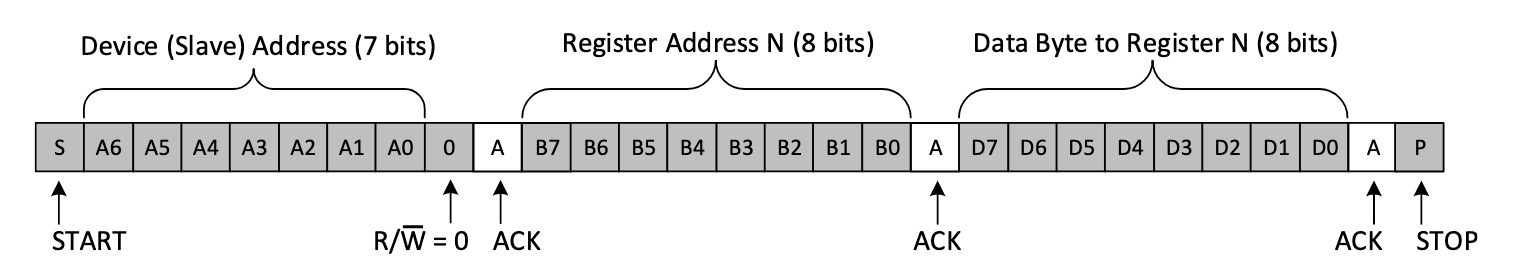
\includegraphics[width=0.8\linewidth]{write.png}
	\caption[I2C Beispiel Schreiben ins Slave Device's Register]{I2C Beispiel Schreiben ins Slave Device's Register}
	\label{fig:write}
	\source{Quelle: \cite{ti.i2c_bus}(S. 7)}
\end{figure}\\
\begin{figure}[!hb]
	\centering
	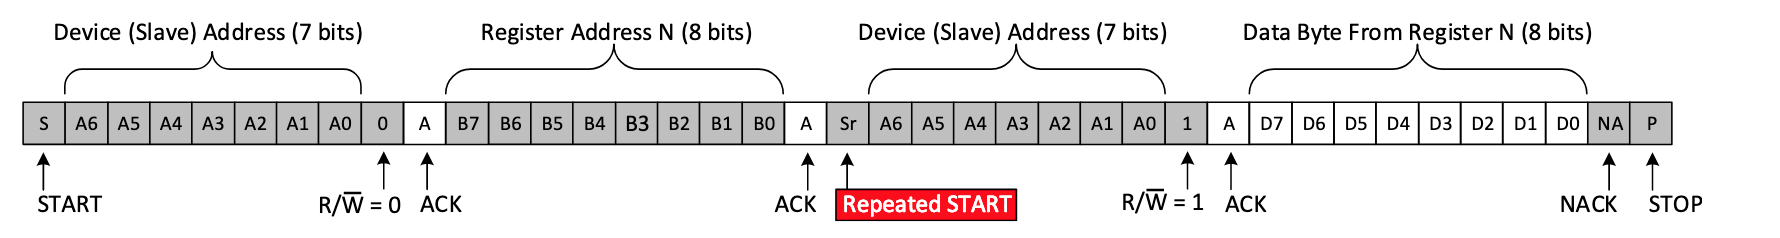
\includegraphics[width=1\linewidth]{read.png}
	\caption[I2C Beispiel Lesen vom Slave Device's Register]{I2C Beispiel Lesen vom Slave Device's Register}
	\label{fig:read}
	\source{Quelle: \cite{ti.i2c_bus}(S. 7)}
\end{figure}\\

Im \textbf{Master-Empfängermodus} werden einige Datenbytes von einem Slave-Sender empfangen. Die Übertragung wird wie im Mastersender-Modus initialisiert. Wenn die Startbedingung übertragen wurde, muss die Interrupt-Service-Routine I2DAT mit der 7-Bit-Slave-Adresse und dem Datenrichtungsbit (SLA + R) laden. Wenn die Slaveadresse und das Datenrichtungsbit gesendet und ein Bestätigungsbit empfangen wurde, wird das serielle Interrupt-Flag (SI) erneut gesetzt und eine Nummer festgelegt Statuscodes in I2STAT sind möglich. Die Abbildung \ref{fig:read} zeigt das Lesen vom Slave's Register.

\subsection{Software}
Die Slave-Adresse und die zu sendenden Daten werden in globalen Variablen abgelegt, damit sie vom I2C Interrupt-Routine verwendet werden können. Die Adresse ist eine Sieben-Bit-Adresse, wobei das LSB zum Schreiben eingestellt und zum Lesen gelöscht ist. Als nächstes löscht die Routine die I2C-Steuerflaggen, aktiviert die I2C-Peripherie und gibt eine Startbedingung aus. Nachdem die Startbedingung auf den Bus geschrieben wurde, wird ein Interrupt generiert, und ein Ergebniscode kann aus dem I2C-Statusregister gelesen werden.

\begin{lstlisting}
unsigned int ADXLI2CAdresss = 0x3A;
unsigned char GlobalI2CAddr;
unsigned char GlobalI2CReg;
unsigned char GlobalI2CData;
unsigned char GlobalI2CRead;
\end{lstlisting}

Wenn die Startbedingung erfolgreich war, lautet der Code im I2STAT-Register 0x08. Als nächstes muss die Anwendungssoftware die Slave-Adresse und das R / W-Bit in das I2Cdata-Register schreiben. Wenn die Bestätigung empfangen wird, wird ein weiterer Interrupt generiert, und das Statusregister I2STAT enthält den Code 0x18, wenn die Übertragung erfolgreich war. Nachdem der Slave nun adressiert wurde und bereit ist, Daten zu empfangen, können wir eine Bytefolge in das I2C-Datenregister schreiben. Wenn jedes Byte geschrieben wird, wird es übertragen und bestätigt. Bei Bestätigung wird ein Interrupt generiert und 0x28 befindet sich im Statusregister, wenn die Übertragung erfolgreich war. Wenn es fehlschlug und ein NACK vorhanden war, lautet der Code 0x20 und das Byte muss erneut gesendet werden. Wenn also jedes Byte übertragen wird, wird ein Interrupt generiert, der Statuscode kann geprüft und das nächste Byte gesendet werden. Nachdem alle Bytes gesendet wurden, kann die Stoppbedingung durch Schreiben in das I2C-Steuerregister aktiviert werden, und die Transaktion ist abgeschlossen. Die Abbildung\ref{fig:master_write} und  Abbildung\ref{fig:master_read} zeigen die Zustände, die im I2STAT-Register eintreten werden.

\begin{figure}[!ht]
	\centering
	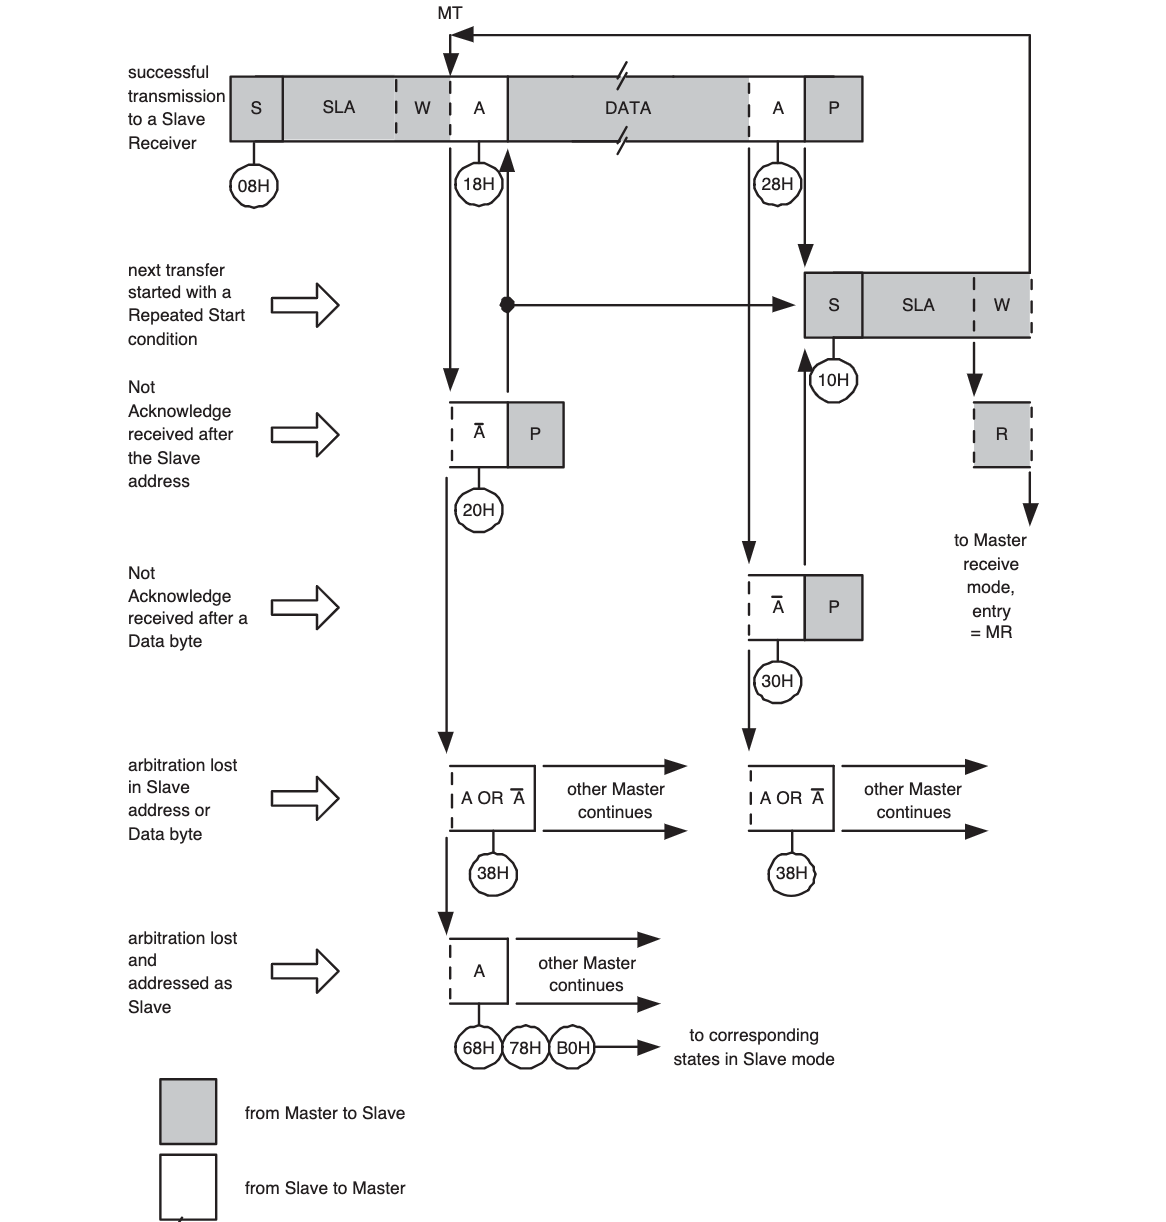
\includegraphics[width=1\linewidth]{master_write.png}
	\caption[I2STAT-Register während Schreiben]{I2C Zustände ins I2STAT-Register während Schreiben}
	\label{fig:master_write}
	\source{Quelle: \cite{nxp.lpc23xx.user_manual}(S. 520)}
\end{figure}
\begin{figure}[!ht]
	\centering
	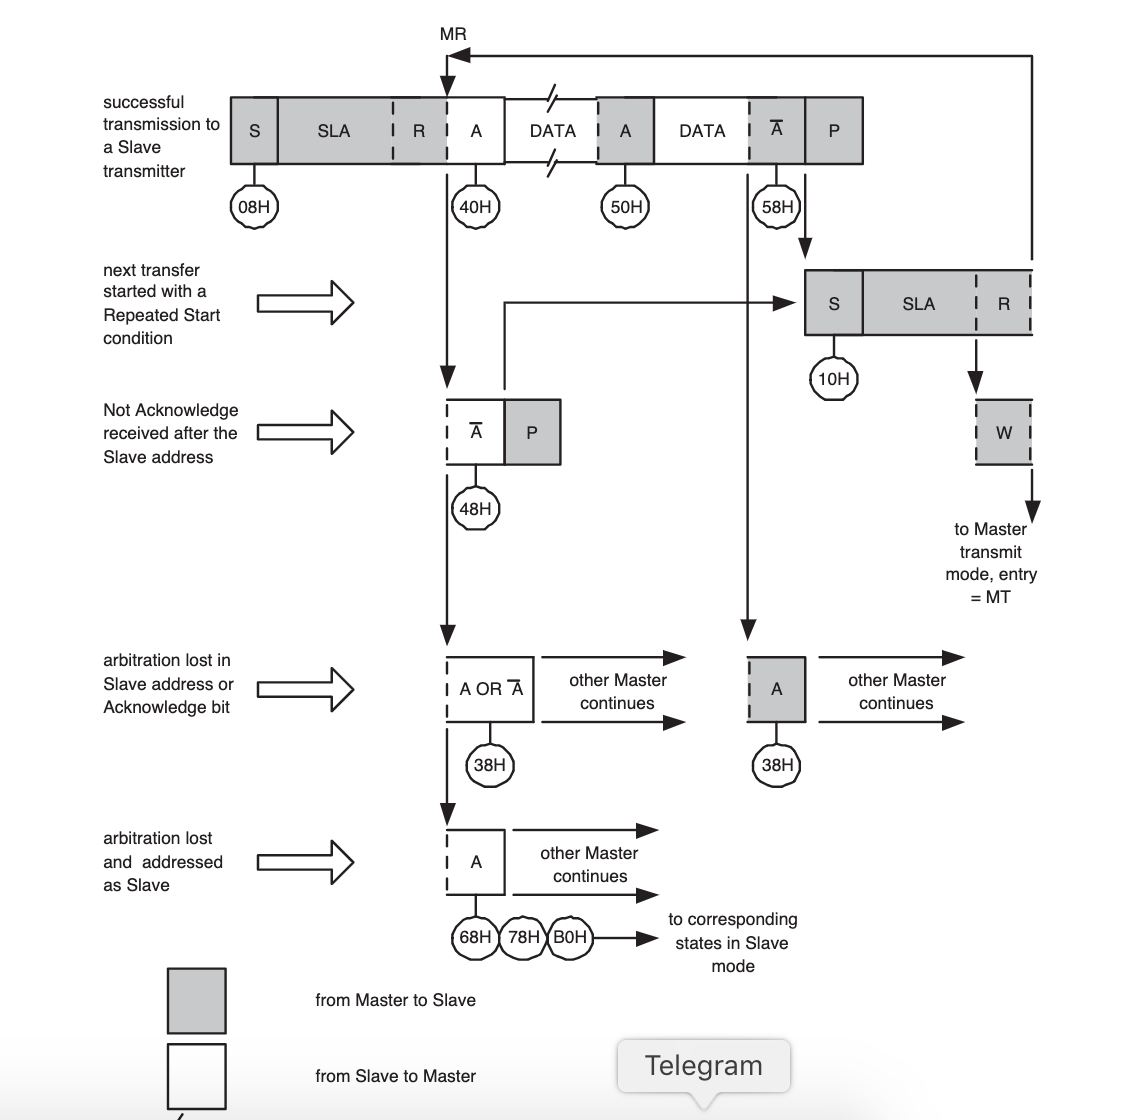
\includegraphics[width=1\linewidth]{master_read.png}
	\caption[I2STAT-Register während Lesen]{I2C Zustände ins I2STAT-Register während Lesen}
	\label{fig:master_read}
	\source{Quelle: \cite{nxp.lpc23xx.user_manual}(S. 521)}
\end{figure}
\clearpage

Um das Lesen des Quellcodes zu vereinfachen, werden die entsprechenden Zuständen als $enum$-type deklariert:
\begin{lstlisting}
volatile enum {
	I2C_IDLE,
	I2C_ADR,
	I2C_STARTED,
	I2C_RESTARTED,
	I2C_REG,
	I2C_DAT,
	I2C_DAT_ACK,
	I2C_RESTART,
	I2C_DAT_NACK,
	I2C_WRITE,
	I2C_READ,
	I2C_ERR,
	I2C_LOST,
	I2C_DONE
} GlobalI2CState;
\end{lstlisting}

Um die gemessene Daten vom dem Beschleunigungsmesser ADXL345 zu lesen, werden die 6  Register verwendet. Die I2C Interrupt Service Routine wird erweitert und damit ein Mehrbyte-Lesen von 2 Register durchgeführt. Die Ausgangsdaten sind zwei Komplemente, mit DATAx0 als niedrigstwertigem Byte und DATAx1 als höchstwertigem Byte, wobei x X, Y oder Z darstellt. 
\begin{lstlisting}
unsigned char XRegs[] = {ADXL345_REG_DATAX0, ADXL345_REG_DATAX1};
unsigned char YRegs[] = {ADXL345_REG_DATAY0, ADXL345_REG_DATAY1};
unsigned char ZRegs[] = {ADXL345_REG_DATAZ0, ADXL345_REG_DATAZ1};
\end{lstlisting}
	
Der I2C-Interrupt ist einfach eine Zustandsmaschine, die das Statusregister für jeden Interrupt untersucht und die erforderliche Aktion ausführt. Dies kann als SWITCH-Anweisung implementiert werden, wie unten gezeigt.
\begin{lstlisting}
__irq void i2c_irq(void) {
	switch (I21STAT) // Read result code and switch to next action
	{
	case (0x08): // A START condition transmitted. Next: 0x18
		// Case ADR -> STARTED
		I21CONCLR = 0x20; // Clear start bit
		I21DAT = GlobalI2CAddr; // Send address and write bit R/W = 0.
		I21CONSET = 0x04; // Write 0x04 to I2CONSET to set the AA bit
		I21CONCLR = 0x08; // Clear SI flag
		GlobalI2CState = I2C_STARTED;
		break;
	
	case (0x10): // A repeated START condition transmitted. Next: 0x18
		if(GlobalI2CState == I2C_READ) {
		// Write Slave Address with R/W bit to I2DAT
		I21DAT = GlobalI2CAddr | 1; // Send address and read bit R/W = 1
		}
		if(GlobalI2CState == I2C_WRITE) {
		// Write Slave Address with R/W bit to I2DAT
		I21DAT = GlobalI2CAddr; // Send address and read bit R/W = 0
		}
		I21CONSET = 0x04; // Write 0x04 to I2CONSET to set the AA bit
		I21CONCLR = 0x28; // Clear start bit and SI flag
		break;
		
	// Previous state was State 8 or State 10, 
	// Slave Address + Write has been transmitted, ACK has been received.
	// The first data byte will be transmitted, an ACK bit will be received.
	case (0x18): // Next: 0x28
		// Case STARTED -> REG
		//I21DAT = GlobalI2CReg; // Write data to TX register
		I21DAT = I2CMasterBuffer[ReadIndex]; // Write data to TX register
		//ReadIndex++;
		I21CONCLR = 0x08; // Clear SI bit
		GlobalI2CState = I2C_REG; // with re-start for write
		break;
	
	case (0x20): // SLA+W has been transmitted; NOT ACK has been received
		I21DAT = GlobalI2CData;
		I21CONCLR = 0x08; // clear SI flag
		GlobalI2CState = I2C_DAT;
		break;
	
	case (0x28): // Data byte in I2DAT has been transmitted; ACK has been received.
	case (0x30): // transmitted, NOT ACK has been received
		// Repeated Start for Read Operation
		// Case RESTART -> READ
		if (GlobalI2CState == I2C_REG && GlobalI2CRead) {
			I21CONSET = 0x24; // Repeated start condition for Read Access
			I21CONCLR = 0x08; // clear SI flag
			GlobalI2CState = I2C_READ;
		}
		// Case RESTART -> WRITE
		else if (GlobalI2CState == I2C_REG && !GlobalI2CRead) {
			// with re-start for write
			//I21CONSET = 0x24; // Repeated start condition for Write Access
			//I21CONCLR = 0x08; // clear SI flag
			GlobalI2CState = I2C_WRITE;
		}
		
		if (GlobalI2CState == I2C_WRITE) {
			I21DAT = GlobalI2CData;
			GlobalI2CState = I2C_DAT;
			I21CONCLR = 0x08; // clear SI flag
		}
		else if (GlobalI2CState == I2C_DAT) {
			GlobalI2CState = I2C_DONE;
			I21CONSET = 0x10; // STO
			I21CONCLR = 0x08; // clear SI flag
		}
		break;
		
	case (0x38): // Arbitration lost
		I21CONSET = 0x24; // to set the STA and AA bits
		I21CONCLR = 0x08; // clear SI flag
		GlobalI2CState = I2C_LOST;
		break;
	
	case (0x40) : // SLA+R has been transmitted; ACK received. Next: 0x50
		I21CONSET = 0x04; // Enable ACK for data byte
		I21CONCLR = 0x08; // clear SI flag
		break;
	
	case (0x48) : // Slave Address +R, Not Ack
		I21CONSET = 0x14; // set the STO and AA bits
		I21CONCLR = 0x08; // clear SI flag
		GlobalI2CState = I2C_ERR;
		break;
	
	/* Data has been received, ACK returned. Data read from I2DAT.
	Additional data will be received. If this is the last data byte 
	then NOT ACK will be returned,
	otherwise ACK will be returned */
	case (0x50):
	case (0x58): // Data Received, Not Ack
		if (ReadIndex != ReadLenght) {
			GlobalI2CData = I21DAT;
			I2CReadBuffer[ReadIndex] = I21DAT;
			ReadIndex++;
			I21CONCLR = 0x0C; //clear the SI flag and the AA bit
			GlobalI2CState = I2C_DAT_ACK;
		}
		else {
			ReadIndex = 0;
			I21CONSET = 0x10; // set STO
			GlobalI2CState = I2C_DONE;
		}
		I21CONCLR = 0x08; // clear SI flag
		break;
	
	default:
		break;
	}	
	VICVectAddr = 0x00000000; // Clear interrupt in
}
\end{lstlisting}

Das Schreiben wird vom Lesen mithilfe des Flags $GlobalI2CRead$ unterscheidet. Wird $GlobalI2CRead$ von Software auf 1 gesetzt, wird dann die wiederholte START-Bedingung erzeugt und I2C-Interrupt wird mit dem Zustand $0x10$ gesetzt und das Lesen wird durchgeführt. 

\begin{lstlisting}
void I2CWriteReg(unsigned char addr, unsigned char reg, 
unsigned char data) {
	...
	GlobalI2CData = data;
	GlobalI2CRead = 0;
	GlobalI2CState = I2C_ADR;
	I21CONSET = 0x20; // Start condition
}
\end{lstlisting}

\begin{lstlisting}
uint16_t I2CRead16Bits(unsigned char addr, unsigned char regs[])  
{
	...
	GlobalI2CRead = 1;
	GlobalI2CState = I2C_ADR;
	I21CONSET = 0x20; // Start condition
}
\end{lstlisting}

Es wird im I2C Zustand $0x28$ unterscheidet, ob es Lesen oder Schreiben durchführen werden sollen.
\begin{lstlisting}
if (GlobalI2CState == I2C_REG && GlobalI2CRead) {
     // Case RESTART -> READ
	I21CONSET = 0x24; // Repeated start condition for Read Access
	I21CONCLR = 0x08; // clear SI flag
	GlobalI2CState = I2C_READ;
}
// Case RESTART -> WRITE
else if (GlobalI2CState == I2C_REG && !GlobalI2CRead) {
	//I21CONCLR = 0x08; // clear SI flag
	GlobalI2CState = I2C_WRITE;
\end{lstlisting}

Nach dem wiederholten Start-Bedingung wird es nach dem Zustand $0x10$ gewechselt und dann den Flag für Lesen auf 1 gesetzt:
\begin{lstlisting}
if(GlobalI2CState == I2C_READ) {
	// Write Slave Address with R/W bit to I2DAT
	I21DAT = GlobalI2CAddr | 1; // Send address and read bit R/W = 1
}
\end{lstlisting}

Nach der Implementierung alle oben genannten Verfahren, werden die gemessene Daten vom digitalen Beschleunigungsmesser ADXL345 angelesen. Die abgelesene Daten können weiter in Programm verwendet werden und die Position von Komponenten der LED-Panels ansteuern.

